\documentclass[../pfc.tex]{subfiles}

\begin{document}
	
	\section{Estructura y descripción de los contenidos de CDROM}
	
	Según la normativa de entrega de documentación de proyectos, los contenidos alojados en el CDROM que acompaña a la memoria de proyecto 'APLICACIÓN COMPLEMENTARIA A LA INICIATIVA DE LA AECC DIARIO DE UN SUPERVIVIENTE' son los siguientes;
	
	\begin{itemize}
		\item La versión en PDF del documento impreso completo bajo el nombre 'memoria.pdf'.
		\item Carpeta con el código fuente de la aplicación llamada 'CodigoFuente'.
		\item La versión instalable de la aplicación con el nombre 'diario.apk'.
		\item La versión electrónica del manual de uso dentro de la carpeta 'ManualUsuario'
		\item Documentación adicional relevante dentro de la carpeta 'OtraDocumentacion'
	\end{itemize}
	
	\begin{figure}[H]
		\centering
		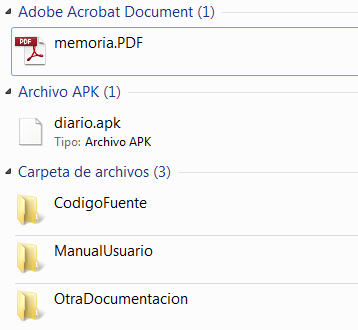
\includegraphics[width=0.6\linewidth]{../images/contenidoCD}
		\caption{Estructura del contenido del CDROM}
		\label{fig:cleanarch}
	\end{figure}
	
\end{document}